\section{Regelung}


Die in Abschnitt \ref{cha:modell} vorgestellten Modellierungsansätze haben den Zweck, ein reales System, wie z.B. die 3D-Servo-Presse, in ein Ersatzmodell zu überführen. Dieses hat den Zweck, einen möglichst guten mathematischen Zusammenhang zwischen den Eingangs- und Ausgangsgrößen des realen Systems zu liefern. \\
Nach \cite{Lunze.2013} wirken Eingangsgrößen (z.B. Spindel- und Exzentervorschübe) auf das System ein und verursachen zeitliche Veränderungen des Systems. Die Ausgangsgrößen (z.B. die Position des Stößels) dagegen beschreiben das Systemverhalten als Reaktion auf die Eingangsgrößen. Da sich dabei Kenngrößen des Systems zeitlich verändern, ergibt sich für solchen der Begriff \textit{Dynamisches System}. Nach \cite{Lunze.2013} besteht die Aufgabe der Regelungstechnik nun darin, für ein solches dynamisches System die beeinflussbare Größe $u(t)$ (Stellgröße bzw. Eingangsgröße) so anzupassen, dass ein Regelungsziel $w(t)$ (Führungsgröße bzw. Sollwert) erreicht wird, siehe Abbildung \ref{fig:regelkreis}.

\begin{figure} 
	\centering
	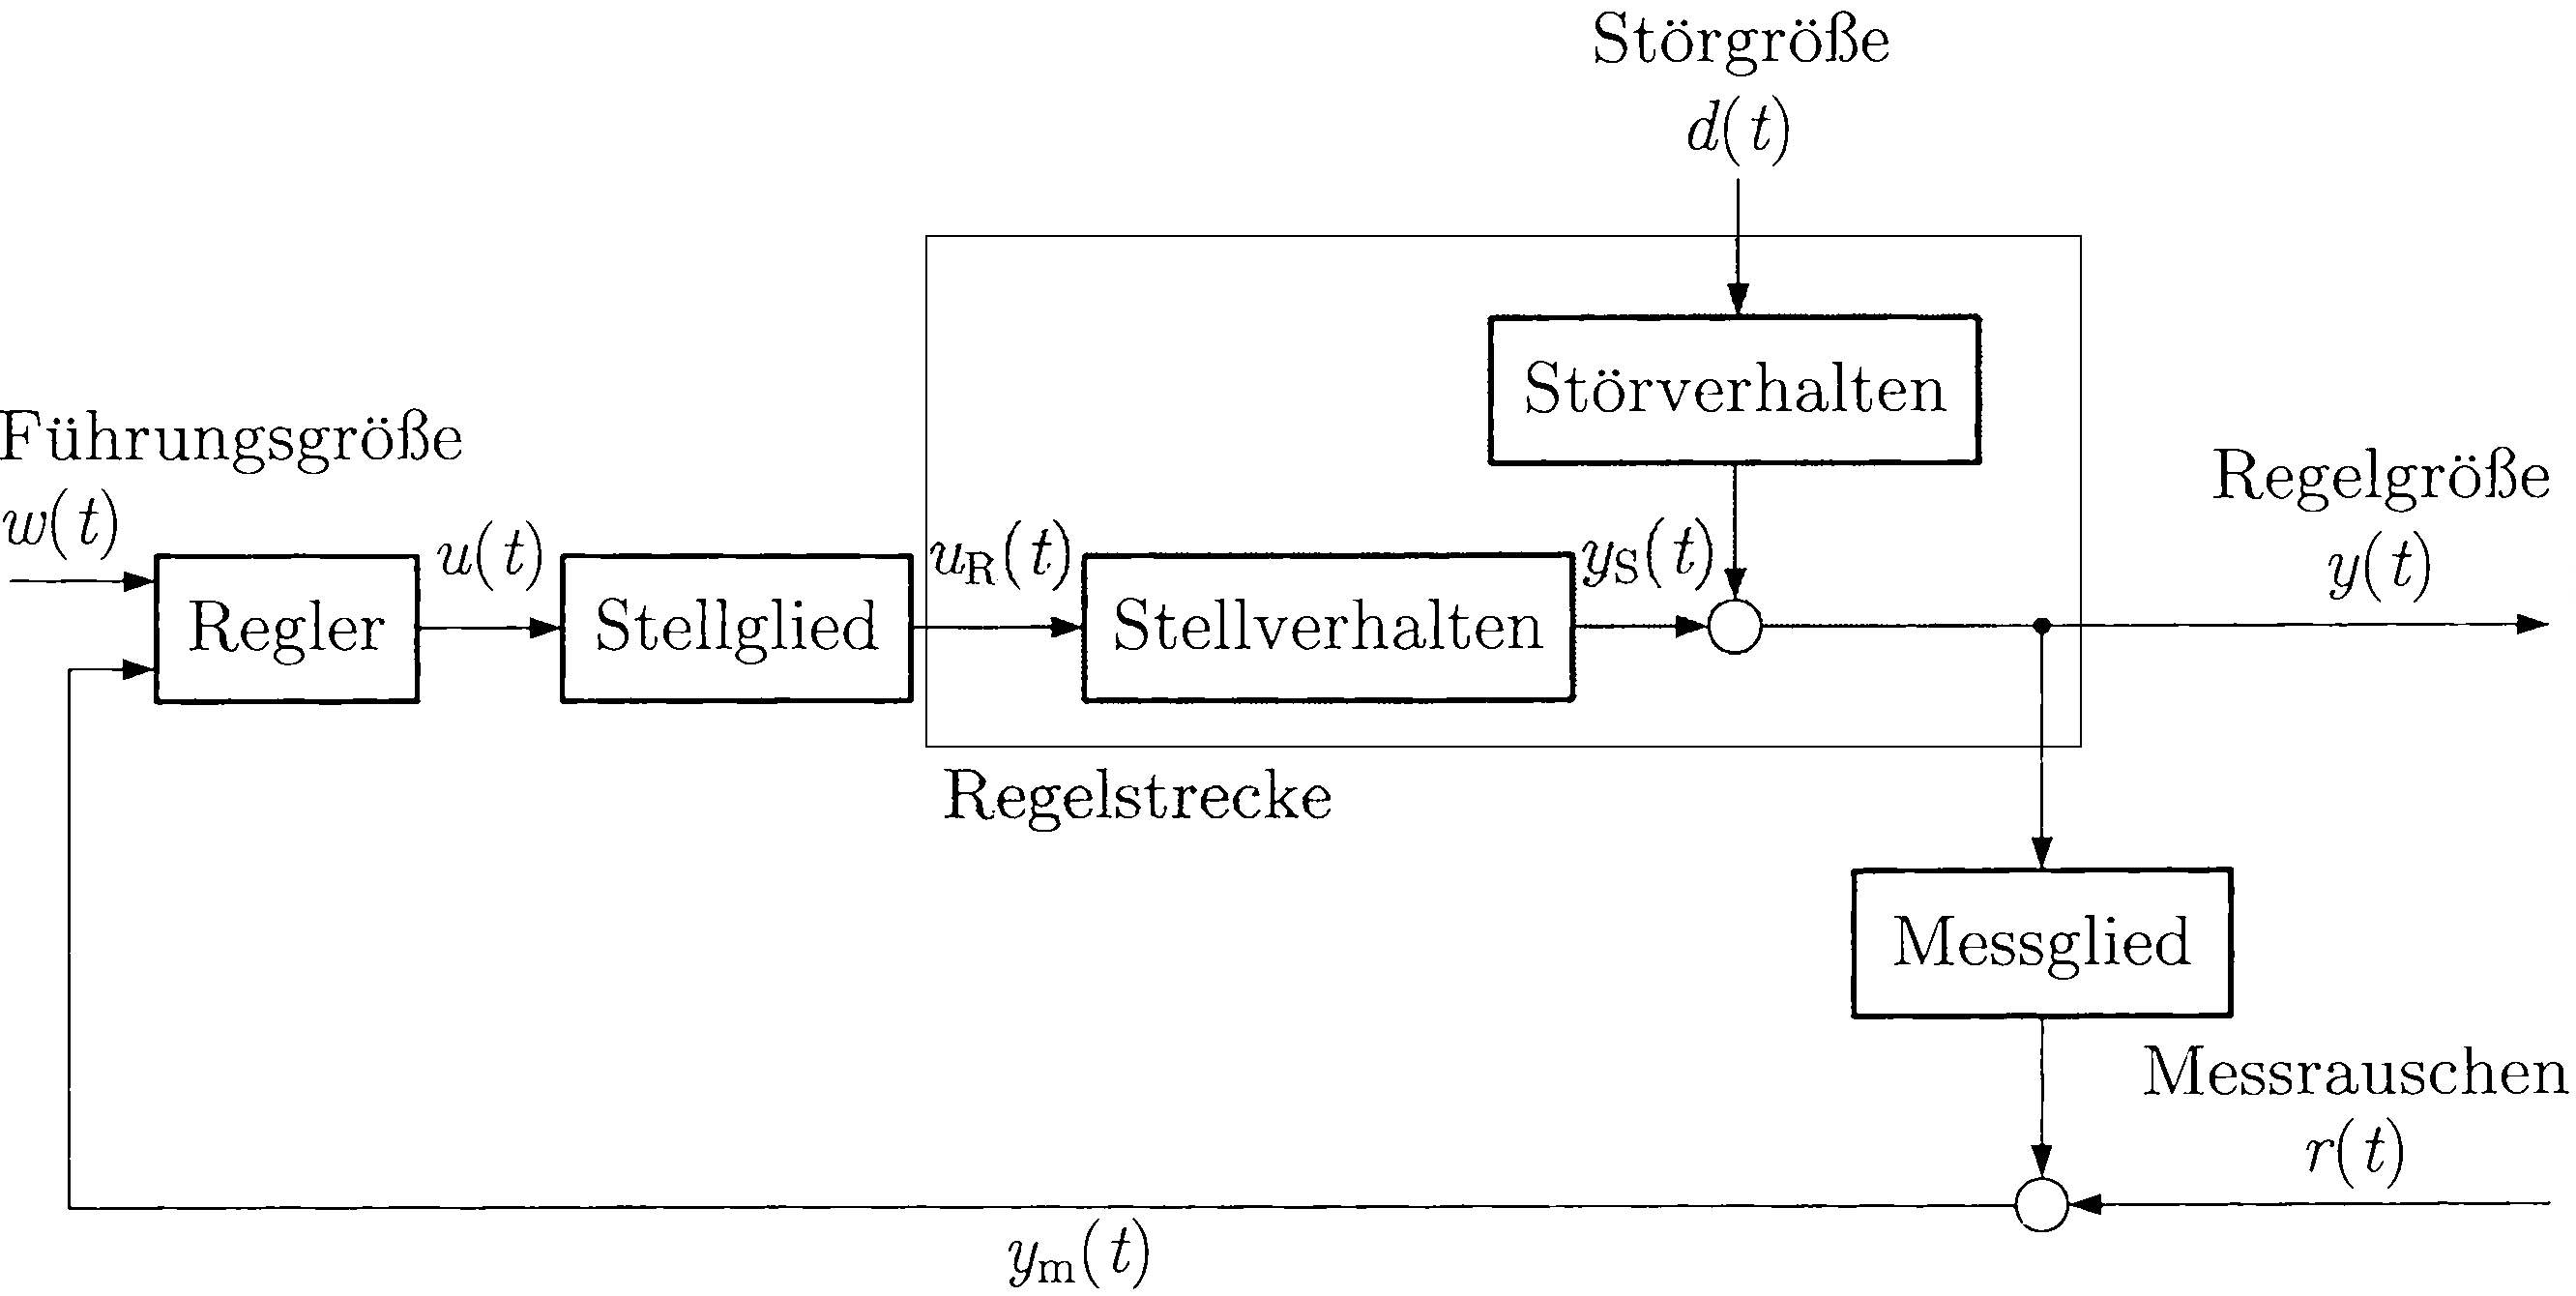
\includegraphics[width=0.75\textwidth]{images/Regelkreis}
	\caption{Erweiterte Grundstruktur des Regelkreises \cite{Lunze.2013}}
	\label{fig:regelkreis}
\end{figure}




Dabei erfüllt die Regeleinrichtung die Aufgabe, unter Nutzung der gemessenen Werte für die Regelgröße (Ausgangsgröße) $y(t)$ die Stellgröße (Eingangsgröße) $u(t)$ so vorzugeben, dass die Differenz zwischen der gemessen Regelgröße (Ausgangsgröße) $y(t)$ und Führungsgröße $w(t)$ minimal ist.  Die Bezeichnung dieser Differenz lautet Regelabweichung $e(t)$, anhand derer die Regeleinrichtung die Stellgröße $u(t)$ zweckmäßig vorgibt. \cite{Lunze.2013}
  
\begin{equation}
e(t) = w(t) - y(t)
\end{equation}


Laut \cite{Lunze.2013} gibt es häufig eine Differenz zwischen der Regelgröße $y(t)$ und der gemessenen Regelgröße $y_m(t)$, da das Messglied selbst über dynamische nichtlineare Eigenschaften verfügt. Dasselbe gilt für Stellglieder (z.B. ein Servomotor, welcher eine Spindel antreibt), welche darüber hinaus sich häufig durch dynamisches Verhalten auszeichnen. Als Resultat ergibt sich daraus eine Differenz zwischen der vorgegeben Stellgröße $u(t)$ und der für den Prozess wirksamen Stellgröße $u_R(t)$. Diese verursacht eine zeitliche Veränderung des Systems (z.B. Stößelbewegung) und erzeugt somit ein Stellverhalten, welches sich mit einem Störverhalten, hervorgerufen durch die unbekannte Störgröße $d(t)$, überlagert. \cite{Lunze.2013} \\ 
Die Auslegung der Regelstrecke muss nun derartig gestaltet sein, dass sie trotz des dynamischen Verhaltens von Messgliedern und Stellgliedern eine minimal mögliche Differenz zwischen der Regelgröße $y(t)$ und Führungsgröße $w(t)$ einstellt. Dafür ist die Auslegung des Reglers entscheidend. \\ 
Für die Auslegung des Reglers ist der Einsatz von Ersatzmodellen notwendig, welche das Systemverhalten des realen Systems so gut wie möglich abbilden. Wie bereits in Abschnitt \ref{cha:Abgrenzung} diskutiert, ist der Einsatz von White-Box-Modellen als Ersatzmodell mit Problemen verbunden. Diese versuchen durch Modellvereinfachungen das Systemverhalten mathematisch zu beschreiben. Damit können sie aber maximal das Stellverhalten des Systems, aber nicht das durch die unbekannte Störgröße $d(t)$ hervorgerufene Störverhalten abbilden. Black-Box-Modelle dagegen, welche mit den Methoden des maschinellen Lernens parametrisiert sind, können auch das Störverhalten mit abbilden, da die Parametrisierung über gemessene Daten stattfindet. Ein Black-Box-Modell, welches das reale Systemverhalten genau genug beschreibt, kann neben der Auslegung von Reglern oder als Hilfsglied im Regelkreis auch im Bereich der Zustandsüberwachung zum Einsatz kommen. Die Grundlagen der Zustandsüberwachung sind im nächsten Abschnitt erläutert.




